\documentclass[output=paper
,modfonts
,nonflat]{langsci/langscibook} 

\title{Labeling, selection, and feature checking}
\author{%
 Hedde Zeijlstra\affiliation{Georg-August-University Göttingen}
}

\abstract{In this paper, I sketch the outlines of an approach to labeling, selection and feature checking that brings minimalist syntax closer to categorial grammar. The central idea is that the distribution of every syntactic element is fully determined by the unordered set of its independent and dependent formal features. Upon merger, every feature on both of the merged elements percolates, unless an independent feature [F] and a dependent feature [uF] stand in a sisterhood relation; then, neither of these two features percolate. This provides a proper labeling algorithm that can also account for the labeling of adjunction. The proposal further reinstalls c-selection and explains the effects traditionally attributed to structural case in terms of DP-selection. It also reduces the set of categorial features to a few primitive independent features ([D], [T], [Pred]). In the final part of this paper, it is discussed how this proposal relates to, or even derives, syntactic operations, such as Agree, movement or valuation. }

\begin{document}
	\maketitle

\section{Labeling: The question}
\subsection{Projection by selection}
Since \citet{Chomsky1995}, labeling has become a widely discussed topic within minimalist syntax. Since, Merge applies to features, labeling amounts to determining what feature should appear on the top node. The central question has been if, why, and how the merger of F and G, \{F, G\}, should receive a label. What is it that determines what needs to be inserted in the \ul{} slot in (\ref{ex-zeijlstra:1})?

\begin{figure}[!h]
\begin{exe} 
\exbox{\label{ex-zeijlstra:1}
	\begin{forest}	
		[ \ul{}
		[F]
		[G] ]
	\end{forest}}
\end{exe} \vspace{-1.3cm}
\end{figure}
\newpage\noindent In \citet{Chomsky1995}, it was argued that, in every instance of Merge, the selector would project its (categorial) features to the top node, a position further elaborated by \citet{Adger2003} (see also \citealt{Boeckx2008} and \citealt{Cecchetto_Donati2010} for similar proposals). Under this approach what selects projects. Canonical cases of projection by selecting heads are presented in (\ref{ex-zeijlstra:2}) (for the sake of convenience denoted in bracket and traditional X-bar notations). 

\begin{exe}
\ex Head–complement configurations \label{ex-zeijlstra:2}
	\xlist
	\ex {[} \textsubscript{V'} {[}V DP{]}{]} \label{ex-zeijlstra:2a}
	\ex {[} \textsubscript{D'} {[}D NP{]}{]} \label{ex-zeijlstra:2b}
	\ex {[} \textsubscript{P'} {[}P DP{]}{]} \label{ex-zeijlstra:2c}
	\endxlist
\end{exe}
In (\ref{ex-zeijlstra:2a}), the verb’s theta-grid selects an internal argument; hence V (or, to be more precise, the feature {[}V{]}), having merged with DP (or more precisely, an element carrying [D]), has its theta-requirement satisfied, and thus projects up to the top node (yielding a feature {[}V{]} at the top node). Similarly, in (\ref{ex-zeijlstra:2b}), D selects for an NP-complement, and in (\ref{ex-zeijlstra:2c}), P selects for a DP-complement. Since V, D, and P are the selectors, V, D, and P (or, to be more precise, the {[}V{]}, {[}D{]} and {[}P{]} features) percolate up.

A major advantage of such a labeling mechanism is that it is not restricted to head-complement relations (see \citealt{Adger2003}). Also, the label of what is traditionally referred to as the merger of a specifier and a bar-level is captured under this approach, both for elements that are base-generated in and for elements that are raised into the specifier position, as is shown in (\ref{ex-zeijlstra:3}).

\begin{exe}
	\ex Specifier–head–complement configurations \label{ex-zeijlstra:3}
	\xlist
	\ex {[} \textsubscript{vP} D{[} \textsubscript{v'} v VP{]}{]} \label{ex-zeijlstra:3a}
	\ex {[} \textsubscript{TP}{[} \textsubscript{T'} T vP{]}{]} \label{ex-zeijlstra:3b}
	\endxlist
\end{exe}
In (\ref{ex-zeijlstra:3a}), v first merges with VP and then this merger merges with DP (in the specifier position). Since it is v that selects both its VP-complement and its DP-specifier, it is v that projects in both cases. In cases of Internal Merge, the same principle applies. In (\ref{ex-zeijlstra:3b}), T selects for a verbal complement (either vP or VP) and for a DP in its specifier position. Since T’s selectional requirements have been met by means of External Merge with vP and Internal Merge with DP, the label of the entire constituent is again T.

At the same time, there are various challenges that such a labeling approach faces and that have given rise to a variety of alternatives to this approach. In this paper I will discuss what I consider the six major challenges against the view on labeling that say that what selects projects. However, I will not argue that, as is currently often done, this should call for an alternative view on labeling. Rather, I will present a view on labeling and selection, building forth on insights presented in \citet{Adger2003}, that derives projection by selection by assuming that upon Merge every feature of both merged elements percolates, unless a pair of matching interpretable and uninterpretable features stand in a sisterhood relation; then neither of these two features percolate. In this paper I argue that such an account of labeling remedies the challenges (and even a few more problems) that the original selection by projection approach faces.

\subsection{Six challenges} \label{sec-zeijlstra:1.2}
Despite these advantages, \textit{projection by selection} as labeling algorithm has currently been replaced by other alternatives (cf. \citealt{Collins2002}, \citealt{Chomsky2008, Chomsky2013, Chomsky2015}). This is partially due to the fact that \textit{selection by projection} faces at least six major challenges. In short, these are: 

\begin{exe}
\ex Challenges for \textit{projection by selection}:
	\xlist
	\ex Motivation
	\ex Adjunction
	\ex Free ordering
	\ex C-selection vs. s-selection
	\ex Mutual selection
	\ex Differences between (long-distance) Agree and local selection.
	\endxlist
\end{exe}
Let’s discuss each challenge in turn. Under the original \textit{selection by projection} approach, the link between projection and selection is not well motivated. Rather, it is stipulated that elements that enter the structure with selectional properties must project. There is nothing in the theory that explains why the selecting element should also be the projecting element.  

Second, even though the original proposal can handle labeling of both head–complement configurations and of the merger between a specifier and a bar-level (in traditional terms), labeling of adjuncts is not captured by it. Adjuncts are problematic for this proposal in two ways. First, if the label of the merger of an adjunct and some element X has the same label as X itself, the adjunct should have been selected by X, but adjuncts, by definition, are not selected by the elements they modify. A second problem is that (phrasal) adjuncts modify elements that count as maximal projections but then continue to project. Why is X in (\ref{ex-zeijlstra:5}) allowed to further project \textit{after} merging with the adjunct if it already acts at as a maximal projection \textit{before} merging with the adjunct?  

\begin{exe}
\ex Adjunction \label{ex-zeijlstra:5} \\
	{[} \textsubscript{X-MAX} YP{[} \textsubscript{X-MAX} XP{]}{]}
\end{exe}
For these and other reasons, adjuncts are often left out of the core structure of sentences, and are said to undergo late merger (cf. \citealt{Lebeaux1988}) or not to establish regular mergers with their modifiees (cf. \citealt{Chomsky2001}; \citealt{Hornstein_Nunes2009}). This way, their unexpected phrasal status no longer forms a problem for the general labeling algorithm, but, of course, the question is left open as to what generates the label of an adjunct and its sister, and why adjuncts are exceptional in this sense.

A third challenge for \textit{projection by selection} concerns the ordering of mergers (cf. \citealt{Adger2013}). Looking again at (\ref{ex-zeijlstra:3}), what would prevent structures like {[}\textsubscript{vP} VP {[}\textsubscript{v'} v DP{]}{]} or {[}\textsubscript{TP} vP {[}\textsubscript{T'} T DP{]}{]}, where the head v/T takes a DP-complement and where VP/vP end up in the specifier position? Such vPs/TPs should of course be ruled out, but if projection simply results from selection, and selectional requirements are not ordered on functional heads, nothing forbids such constructions.

Perhaps more importantly, one of the core cases of selection, namely theta-role assignment, has nowadays been relegated to the domain of semantics. Argument selection rather seems to be a semantic requirement (s-selection) and not a syntactic one (c-selection). This is shown in (\ref{ex-zeijlstra:6}). \textit{Know} needs a complement to which it assigns a theta-role, but the syntactic status of this complement is underdetermined. It can either be a DP, a PP, or a CP. 

\begin{exe}
\ex to know \label{ex-zeijlstra:6}
	\xlist
	\ex {[}\textsubscript{VP} \textit{know} {[}\textsubscript{DP}
		\textit{Mary}{]}{]}
	\ex {[}\textsubscript{VP} \textit{know} {[}\textsubscript{PP} 	
		\textit{about Mary}{]}{]}
	\ex {[}\textsubscript{VP} \textit{know} {[}\textsubscript{CP} 		
		\textit{that Mary has left}{]}{]}
	\endxlist
\end{exe}
This shows that semantic and not syntactic properties of the complement determine whether theta-role assignment can take place or not. But if the verb does not syntactically select its complement, how can syntax determine that it is the selecting element? This would trigger a look-ahead problem. Unless c-selection can be reinstalled in the theory, \textit{projection by selection} cannot account for the labeling of VPs. 

A fifth challenge comes from mutual selection. Take the following structure.

\begin{exe}
\ex Mutual selection \label{ex-zeijlstra:7} \\
	{[}\textsubscript{PP} \textit{with} {[}\textsubscript{DP} \textit{Mary}{]}{]}
\end{exe}
In (\ref{ex-zeijlstra:7}), the preposition \textit{with} selects a DP-complement. This would call for PP being the label of the merger, instead of DP. However, under fairly standard versions of structural case, the case feature of the DP has been checked in return by (in this case) the P-head. Case assignment can also be thought of as a selectional requirement: every DP needs to be assigned structural case. But then one could just as well argue that \textit{Mary} in (\ref{ex-zeijlstra:7}) has selected its case assigner (which is P in this case, and could be v or finite T in other cases). However, the {[}D{]}-feature of \textit{Mary} does not project up.

Finally, more needs to be said about selectional features. Unless one stipulates an independent set of selectional features as part of the set of formal features, selectional features should be reduced to already existing features that encode syntactic dependencies. Such features are well known and are often referred to as uninterpretable or unvalued features. These features have their ‘selectional’ requirements satisfied by means of the operation Agree. Since \citet{Chomsky2001}, however, it is generally assumed that Agree can take place in long-distance fashion, whereas the kind of selectional requirements that are said to be responsible for projection under the \textit{projection by selection} approach can only take place in a strictly local fashion. Hence, either projection should follow from something else, or selectional features should be separated from uninterpretable or unvalued features, even though they both encode formal dependencies.

\subsection{Alternative labeling algorithms}
In short, in order to maintain the \textit{projection by selection} approach, various problems need to be remedied, and it has not become clear so far how this can be achieved. For these and other reasons, various scholars have proposed alternative labeling algorithms.

For instance, \citet{Collins2002} argues that a merger of F and G, as in (\ref{ex-zeijlstra:1}), does not need a label at all. \citet{Chomsky2013, Chomsky2015}, going back to \citet{Chomsky2008}, has argued that there is no uniform labeling algorithm. The label of the merger of two elements may be determined by either relativized minimality (in head–complement configurations), shared features (in specifier–bar-level configurations involving External Merge) or movement (in specifier–bar-level configurations involving Internal Merge, where a moved element cannot be the source of the label in any of its positions). Other labeling algorithms have been proposed by \citet{Cecchetto_Donati2010, Cecchetto_Donati2015}, who argue that, in principle, both daughters can project their features, and \citet{Adger2013}, who argues that labeling is not endocentric at all, and that a label is not projected by its daughters, but ‘read off’ from a functional sequence of formal features.

All these approaches have their benefits, while, at the same time, facing several problems. Unfortunately, space considerations prevent me from doing full justice to all these proposals by discussing them in detail. What all these proposals share, however, is that they take Merge not to be an operation that inherently gives rise to a label; therefore, either Merge should apply in a labelless way (as Collins has proposed) or an additional labeling algorithm has to be formulated in order to prevent structures from appearing without labels – either for formal reasons or because such structures would be banned at the interfaces. It is, however, questionable whether Merge is indeed an operation that does not inherently yield labels.

\section{Proposal}
\subsection{Labeling, Merge, and feature percolation}
Let’s look again at the case where F and G merge. Under the conception of the above-mentioned theories, Merge applies as in (\ref{ex-zeijlstra:8}), leaving a position (\ul{}) to be filled by a label. The question addressed in all current approaches to labeling then is if, why, and how the merger of F and G, \{F, G\}, should receive a label.

\begin{figure}
	\begin{exe}
		\exbox{ \label{ex-zeijlstra:8}
		\begin{forest}	
			[\ul{}
			[F]
			[G] ]
		\end{forest}}
	\end{exe} \vspace{-0.8cm}
\end{figure}
\noindent But there is a different view on Merge. If Merge combines two sets of formal features, why would this not be a set that contains all formal features that the merged elements consist of? Why is merger of F and G not the union of the feature sets of F and G? In other words, why is the label not F, G or, in set-theoretical terms, F$\cup$G, as in (\ref{ex-zeijlstra:9})?

\begin{figure} 
	\begin{exe}	
\exbox{ \label{ex-zeijlstra:9}
		\begin{forest}	
			[F$\cup$G
			[F]
			[G] ]
		\end{forest}}
	\end{exe} \vspace{-0.8cm}
\end{figure}
\noindent The idea that all features percolate up to the top node is in a way the mirror image of the Inclusiveness Condition, which states that the output of a system does not contain anything beyond its input \citep[225]{Chomsky1995}. Given Inclusiveness, no new material may be included in the tree except for the input from the lexicon. But Inclusiveness can be said to follow from a more general constraint according to which formal information should neither disappear nor be added in the structure (see also \citealt{Neeleman_VanDerKoot2002}). It would then follow that in principle all features percolate up, unless there is a mechanism where the features of one daughter prevent the features of the other daughter to percolate. If the labels in the structures in (\ref{ex-zeijlstra:2}) are indeed correct, a mechanism would then be needed under this approach that makes the features of the sisters of V, D and P not percolate. 

\subsection{Formal and categorial features}
In order to see whether a principled mechanism is available where features can prevent other features to percolate, one should first identify the types of formal features available. In the aftermath of the introduction of the Minimalist Program, various types of features have been proposed: categorial features, selectional features, interpretable and uninterpretable features, edge features, EPP-features, fully uninterpretable features, etc. Naturally, under any minimalist perspective, the taxonomy of formal features should be reduced as much as possible. One attempt in doing so is to unify (un)interpretable features with categorial features. \citet{Zeijlstra2014} argues that the set of (un)interpretable features does not intersect with the set of semantic features, as \citet{Chomsky1995} had proposed. For Zeijlstra, unlike Chomsky, interpretable formal features are purely formal features that have the capacity to check off uninterpretable features, but that lack any semantic interpretation. The fact that elements with a particular formal feature {[}iF{]}, sometimes also denoted as {[}F{]}, often also carry the semantics of F (e.g., an element with particular interpretable formal $\varphi$-features also often, but not always, receives a semantic interpretation of these $\varphi$-features), he takes to be a result of a learnability algorithm, which states how such formal features are acquired. Evidence for this more indirect correspondence between formal and semantic features comes from mismatches between the two (e.g. an element that carries a formal plural feature, but receives a singular semantic interpretation). The taxonomy of formal (un)interpretable features and semantic features would then be as in (\ref{ex-zeijlstra:11}), and not as in (\ref{ex-zeijlstra:10}), which reflects Chomsky’s original proposal:

\begin{figure}[!h]
\begin{exe}
\ex \hspace{1.5cm} Formal Features \hspace{0.8cm} Semantic Features \label{ex-zeijlstra:10} \\
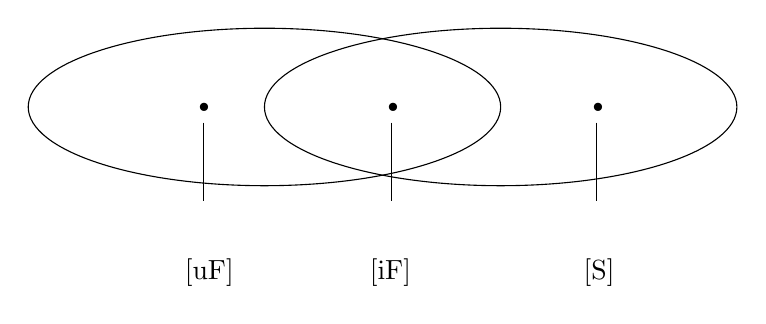
\begin{tikzpicture}
\draw (2,2) ellipse (3cm and 1cm);
\node [right] at (1,2) {\huge{\textbf{.}}};
\node [right] at (3.4,2) {\huge{\textbf{.}}};
\draw (5,2) ellipse (3cm and 1cm);
\node [right] at (6,2) {\huge{\textbf{.}}};
\draw [black] (1.23,1.8) -- (1.23,.8);
\node [below] at (1.3,0.2) {{[}uF{]}};
\draw [black] (3.61,1.8) -- (3.61,.8);
\node [below] at (3.6,0.2) {{[}iF{]}};
\draw [black] (6.22,1.8) -- (6.22,.8);
\node [below] at (6.25,0.2) {{[}S{]}};
\end{tikzpicture}
\end{exe} \vspace{-0.5cm}
\end{figure}
\begin{figure}[!h]
\begin{exe}
\ex \hspace{1.5cm} Formal Features \hspace{2.5cm} Semantic Features \label{ex-zeijlstra:11}\\ 
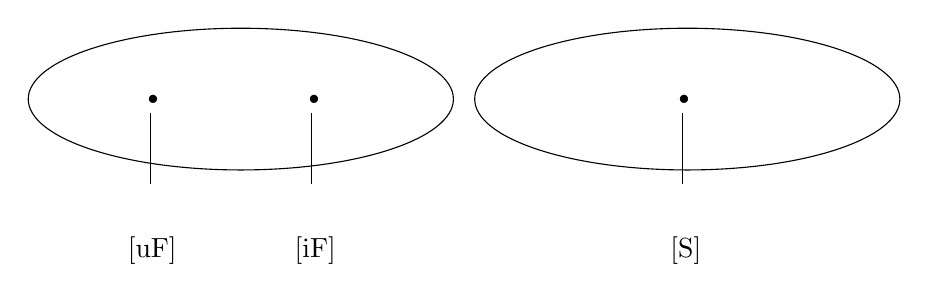
\begin{tikzpicture}[scale=0.9]
\draw (2,2) ellipse (3cm and 1cm);
\node [right] at (0.5,2) {\huge{\textbf{.}}};
\node [right] at (2.78,2) {\huge{\textbf{.}}};
\draw [black] (0.73,1.8) -- (0.73,.8);
\draw (8.3,2) ellipse (3cm and 1cm);
\node [right] at (8,2) {\huge{\textbf{.}}};
\node [below] at (0.75,0.2) {{[}uF{]}};
\draw [black] (3,1.8) -- (3,.8);
\node [below] at (3.05,0.2) {{[}iF{]}};
\draw [black] (8.23,1.8) -- (8.23,.8);
\node [below] at (8.28,0.2) {{[}S{]}};
\end{tikzpicture}
\end{exe} \vspace{-0.8cm}
\end{figure}
\newpage \noindent The major distinction between the proposals in (\ref{ex-zeijlstra:10}) and (\ref{ex-zeijlstra:11}) is that in (\ref{ex-zeijlstra:11}), unlike (\ref{ex-zeijlstra:10}), both types of formal features lack semantic content. Consequently, the only thing that such formal features determine is the syntactic behavior of the elements that they are part of. But if that is the case, such formal features are the same as categorial features, which also lack semantic content and also only determine the syntactic behavior of the elements that they are part of. This does not only apply to what are called interpretable formal features, but also to what are called uninterpretable features. These names are actually misnomers. A more proper way to refer to them would be using ‘independent’ and ‘dependent’ formal or categorial features. Independent features determine the categorial status in a traditional way (a verb has a feature [V], etc.); dependent features encode dependencies on other features. For instance, a feature [uD] encodes the dependency on an element carrying [D].

But if categorial information comes from the joint set of both dependent and independent features, there is no need anymore to allude to additional selectional features: a selectional feature encodes the requirement to be merged with an element that carries a particular independent feature – and that is exactly what a dependent feature does.

\subsection{Feature checking and feature percolation}
Every lexical item can be said to consist of at least two set of features (ignoring the question whether the set of phonological features is really lexically encoded): semantic features, and formal features, where the latter come about in two types: dependent and independent formal features. Both types of formal features determine the lexical item’s syntactic behavior. Now, let’s see what happens when two elements merge, where merger should fulfill a featural dependency.

Suppose some element $\alpha$ that carries the formal features {[}F{]} and {[}uG{]} merges with an element $\beta$ that carries the formal feature {[}G{]}, where {[}X{]} represents a formal interpretable/independent feature and {[}uX{]} a formal uninterpretable/dependent feature. Now the categorial status of $\alpha$ is that of an element of type F that needs an element of type G to survive. If F is V and G is D, $\alpha$ would be a verb that needs to merge with a DP. The result of merging a verb that needs a DP-complement (say a transitive verb) with such a DP is a verb that no longer needs this DP-complement (an intransitive verb). In categorial terms: after merger, both the dependent feature and the element that satisfies the dependency, are cancelled out against each other. That should not come as a surprise. In fact, the hallmark of categorial grammar is that the combination of the elements a/b and b yield an element of category a, just as, in semantic type theory, the mother of a daughter with type e and a daughter with type <e,t> is of type t. 

Let us therefore formulate the following rule, which essentially integrates the basic tenets of categorial grammar into minimalist syntax:

\begin{exe}
\ex \label{ex-zeijlstra:12}\textbf{Rule 1}: Let A and B be two sets of formal features. If A merges with B, for any pair {[}F{]}--{[}uF{]} such that {[}F{]}$\in$A and {[}uF{]}$\in$B, or {[}F{]}$\in$B and {[}uF{]}$\in$A, neither {[}uF{]} nor {[}F{]} percolates; all other features do percolate.
\end{exe}
Given Rule 1, merger of {[}F{]} and {[}G{]} then immediately yields the required result, as is shown in (\ref{ex-zeijlstra:13}) below.

\begin{figure}[!h]
	\begin{exe}
		\exbox{ \label{ex-zeijlstra:13}
		\begin{forest}	
			[\{{[}F{]}\}
			[\{{[}F{]}{,} {[}uG{]}\}]
			[\{{[}G{]}\}] ]
		\end{forest}}
	\end{exe} \vspace{-0.7cm}
\end{figure}
\noindent Note, though, that if the right sister contains any other feature, say an additional dependent feature, nothing stops this feature from percolating up:

\begin{figure}[!h]
	\begin{exe}
		\exbox{
		\begin{forest}	
			[\{{[}F{]}{,} {[}uK{]}\}
			[\{{[}F{]}{,} {[}uG{]}\}]
			[\{{[}G{]}{,} {[}uK{]}\}] ]
		\end{forest}}
	\end{exe} \vspace{-0.9cm}
\end{figure}
\newpage\noindent One thing that still needs to be prevented, though, is the configuration below, where two independent features would both yield to the top node, giving rise to elements whose syntactic behavior is never attested. One would not want to allow grammar to recursively create novel categories in the course of the derivation.
\begin{figure}[!h]
	\begin{exe}
		\exbox{
		\begin{forest}	
			[*\{{[}F{]}{,} {[}G{]}\}
			[\{{[}F{]}\}]
			[\{{[}G{]}\}] ]
		\end{forest}}
	\end{exe} \vspace{-0.8cm}
\end{figure}
\newline \noindent This, however, can be prevented by assuming a second rule that is very similar to \citet{Pesetsky_Torrego2006}'s Vehicle Requirement on Merge, or \citet{Wurmbrand2014}'s Merge Condition.

\begin{exe}
\ex \label{ex-zeijlstra:16} \textbf{Rule 2}: $\alpha$ merges with $\beta$ iff at least one featural dependency is resolved as a result of this merger.
\end{exe}
Informally, (\ref{ex-zeijlstra:16}) states that Merge must involve feature checking. Note that the proposal spelled out above essentially reinstalls \textit{projection by selection}, albeit in a different way. Everything projects except the selecting and selected features. This also means that the various challenges that \textit{projection by selection} met do apply to this proposal as well. Therefore, it needs to be shown how, under this proposal, those challenges can be overcome. Moreover, even though the proposal, in essence, is very simple, the consequences, as will turn out in the next section, are far from trivial and sometimes also far from intuitive. Let’s therefore look at the application of the proposal now.

\section{Application}
\subsection{Motivation}
As already outlined above, the fact that the selecting element projects is now no longer stipulated but follows directly. Every feature except for the selecting and the selected features project (Rule 1), and that Merge, and therefore feature percolation, may only take place if it leads to resolving a featural dependency. Essentially, selectional requirements that are satisfied result in the satisfier and the satisfiee no longer percolating, as is standardly assumed in categorial grammar. 

\subsection{Labeling configurations} \label{sec-zeijlstra:3.2}
With respect to two of the three labeling configurations in question (head--complement, specifier--bar-level and adjunction), the proposal does not work differently from previous versions of the \textit{projection by selection} approach. Assuming that heads like D or P select by means of carrying an uninterpretable feature that can be checked off by their complements (P contains a feature [uD]; D contains a feature [uN]), the labels of the following configurations are directly accounted for. In (\ref{ex-zeijlstra:17a}), neither [N] nor [uN] percolate up; so the only feature that ends up on the top node is [D]. Similarly, [P] is the only feature that percolates up in (\ref{ex-zeijlstra:17b}); neither [D] nor [uD] do.

\begin{exe}
	\ex Head–complement configurations \label{ex-zeijlstra:17}
	\xlist
	\ex {[}\{\textsubscript{{[}D{]}}\} \label{ex-zeijlstra:17a} {[}D\{\textsubscript{{[}D{]}, {[}uN{]}}\} N\{\textsubscript{{[} N{]}}\}{]}{]}
	\ex {[}\{\textsubscript{{[}P{]}}\} \label{ex-zeijlstra:17b} {[}P\{\textsubscript{{[}P{]}, {[}uD{]}}\} D\{\textsubscript{{[}D{]}}\}{]}{]}
	\endxlist
\end{exe}
Under the assumption that specifiers are secondary selected constituents, the picture can be extended to specifiers, again much in the same vein as the original \textit{projection by selection} approach. To see this, look at the following structures of vP and TP (to ensure that no differences arise due to whether the specifier is externally or internally merged).

\begin{exe}
	\ex Configurations involving specifiers \label{ex-zeijlstra:18}
		\xlist
		\ex {[}D\{\textsubscript{{[}D{]}}\} \label{ex-zeijlstra:18a} {[}v\{\textsubscript{{[}v{]}, {[}uV{]}, {[}uD{]}}\} V\{\textsubscript{{[}V{]}}\}{]}{]}
		\ex {[}D\{\textsubscript{{[}D{]}}\} {[}T\{\textsubscript{{[}T{]}, {[}uv{]}, {[}uD{]}}\} v\{\textsubscript{{[}v{]}}\}{]}{]}
		\endxlist
	\end{exe}
In (\ref{ex-zeijlstra:18a}), v contains two selecting uninterpretable features, [uV] and [uD]. After merging v with VP, the only features percolating up are [v] and [uD] ([V] and [uV] don’t). The next step is merger of the feature set \{[v], [uD]\} with \{[D]\}, resulting in a top node \{[v]\}. In exactly the same manner, merging T, the feature set \{[T], [uv], [uD]\}, first with vP (\{[v]\}) and then with DP (\{[D]\}) will result in a top node with the feature set \{[T]\}.

As discussed in section \ref{sec-zeijlstra:1.2}, now the question naturally arises as to what determines that v first merges with VP (or T with vP) and only then with DP? Why wouldn’t or couldn’t the orderings be the reverse? However, in order to answer that question, it should first be determined whether this problem should be solved within a labeling algorithm at all.

At first sight, there appear to be two kinds of solutions to this problem. The first solution would be to impose an ordering on the selecting features, for instance by assigning ordering diacritics (\{[uV]\}\textsubscript{1}, \{[uD]\}\textsubscript{2}), or to think of features sets as being ordered (\textsubscript{<}\{[uV]\}, \{[uD]\}\textsubscript{>}). The alternative solution would be to say that syntax can deliver both orders. In that case, both [\textsubscript{TP} DP [\textsubscript{T’} T vP]] and [\textsubscript{TP} vP [\textsubscript{T’} T DP]] should be syntactically fine, but only the first, and not the second, can receive a semantic interpretation. Under this view, syntax overgenerates, and the interfaces filter out unwanted structures. Each solution has its benefits, but also comes with clear disadvantages. Ordering solutions require extra complications in the mechanics of the system (either novel subfeatures, or more complex rules of feature percolation). Interface solutions have to allude to existing semantic or phonological modes of interpretation that rule out the unwanted structures, and it is far from clear whether, for every unwanted structure, a semantic/phonological solution is available. For the selection by functional heads, a semantic solution, arguably, is available, as these are in general the result of grammaticalized scopal relations, but in other cases, semantics and or/phonology may not be able to rule out such reverse merger orderings. Note, though, that it is also possible that certain reverse orderings are ruled out for syntax-internal reasons. For instance, if in (\ref{ex-zeijlstra:18}) DP were the complement of v/T and VP/vP its specifier, V-to-v, or v-to-T movement would be forbidden as the target head position (v or T) would not c-command the base positon of the adjoined head (V or v).

However, before further evaluating these two types of solutions, let’s first look at what kind of empirical predictions they make. Ordering solutions require that reverse selectional orderings may never take place. Interface solutions predict that, when two different orderings are semantically or phonologically non-anomalous, both should be fine. This gives the interface solution a step ahead: if it turns out that such flexible orderings do exist, the ordering solution can already be discarded, and the absence of structures like [\textsubscript{TP} vP [\textsubscript{T’} T DP]] or [\textsubscript{vP} VP [\textsubscript{v’} v DP]] should, in turn, be semantically or phonologically ruled out. In section \ref{sec-zeijlstra:3.3}, I show that such flexible orderings can indeed be attested.

This, then, leaves us to adjunction. The question that arises is why the merger of an adjunct, say YP, with another phrase, XP, yields the label XP. To make this more concrete, let’s think of XP as a VP and of YP as an AdvP. Why would merger of VP and AdvP yield a label VP, where both instances of VP are maximal projections? Under the standard \textit{projection by selection} approach, this could never be accounted for. Why would the lowest instance of VP be a maximal projection? And, moreover, to the extent that selection is involved in adjunction, it is the adjunct that needs to stand in a particular configuration with its modifiee, not the other way round. Adverbs need VPs; VPs do not need adverbs. 

The solution to the problem, I think, lies in the fact that every known category is generally thought of as a primitive feature. Adverbs carry [Adv], just like prepositions carry [P] and verbs carry [V]. But it may very well be the case that certain categorial features should be replaced by sets of more primitive features, an idea already entertained in \citet{Chomsky1970, Chomsky1981}. Now, under the assumption that V is indeed a primitive feature (just carrying [V], though see section \ref{sec-zeijlstra:3.7} for a refinement of that assumption), the presented proposal offers a heuristic to determine the featural status of a sister, if the features of the other sister and the mother are known. Abstractly, this is shown in (\ref{ex-zeijlstra:19}): 

\begin{figure}[!h]
	\begin{exe}
		\exbox{ \label{ex-zeijlstra:19}
			\begin{forest}	
				[\{{[}Y{]}\}
				[\{{[}X{]}\}]
				[\{{[}Y{]}{,} {[}uX{]}\}] ]
		\end{forest}}
	\end{exe} \vspace{-0.75cm}
\end{figure} 
\noindent If the top node carries \{[Y]\} and one sister carries \{[X]\}, it must be the case that the other sister carries \{[Y], [uX]\}. Now, adjunction is nothing but an instance where \{[Y]\} is identical to \{[X]\}. But if that is the case, the featural status of the other sister should be \{[X], [uX]\}. 
Turning to our example, an adverb modifying a VP should not be said to carry a feature [Adv], but rather a feature set \{[V], [uV]\}.

\begin{figure}[!h]
	\begin{exe}
		\exbox{
			\begin{forest}	
				[\{{[}\textbf{V}{]}\}
				[\{{[}V{]}\}]
				[\{{[}\textbf{V}{]}{,} {[}uV{]}\}] ]
		\end{forest}}
	\end{exe}
\end{figure} \vspace{-0.75cm}
\noindent Now, everything follows. Not only is it explained why the top node is \{[V]\}, but, more importantly, the fact that the configuration contains two maximal projections of VP is also accounted for. If an adverb carries \{[V], [uV]\} and merges with a feature set \{[V]\}, it is the [V]-feature of the VP and the [uV]-feature of the adverb that cannot percolate up. The only feature percolating up is the (boldfaced) \textbf{[V]} feature on the adverb. But that means that the left sister is a maximal projection (the highest projection of the feature [V]), as is the top node (the highest projection of the feature \textbf{[V]}). Naturally, the question arises how syntax knows which element carrying [V] should raise or receive inflection. In other words, how are verbs distinguished form adverbials, now that they are both taken to carry [V]? I will address this issue in the following subsection.

\subsection{Prepositional adjuncts and selectional ordering} \label{sec-zeijlstra:3.3}
Now, the idea that adjuncts that modify VPs are feature sets \{[V], [uV]\} may work well for adverbs, but does not extend to other verbal adjuncts. Take, for instance, PPs. First, PPs do not only modify VPs, but also NPs ([\textsubscript{NP} \textit{sausages} [\textsubscript{PP} \textit{from Italy}]]) or (predicatively used) APs ([\textsubscript{AP} \textit{afraid} [\textsubscript{PP} \textit{of the doctor}]]). Moreover, PPs cannot be reduced to feature sets \{[V], [uV]\}, as PPs are internally complex. If PPs are feature sets \{[V], [uV]\} these features must have percolated up from the inside.

Let’s first aim at the latter question (What is the internal feature structure of a PP?), and save the former question for later (section \ref{sec-zeijlstra:3.7}). The question that then needs to be addressed is what the consequences are for assuming that PP adjuncts, or at least PP adjuncts modifying VPs, are indeed feature sets \{[V], [uV]\}. In that case, the question emerges as to what prepositions themselves are. Again, our heuristic to determine categorial features can be of help. If PPs are feature sets \{[V], [uV]\}, then Ps must be feature sets \{[V], [uV], [uD]\}.

\begin{figure}[!h]
	\begin{exe}
		\exbox{
			\begin{forest}	
				[PP{=}\{{[}V{]}{,} {[}uV{]}\}
				[P{=}\{{[}V{]}{,} {[}uV{]}{,} {[}uD{]}\}]
				[DP{=}\{{[}D{]}\}] ]
		\end{forest}}
	\end{exe} \vspace{-0.75cm}
\end{figure} 
\noindent Under this view, prepositions are elements that, once merged with a DP, behave like adverbials. That seems only partially correct, though. Prepositions merged with a DP can behave adverbials (like \textit{in the garden} in \textit{Mary is walking in the garden}). However, they can also function as arguments. That means that, unless the argument–adverbial distinction can be encoded somewhere in the syntax (i.e., when it is recognizable which element carrying \{[V], [uV]\} is argumental and which one is not), this proposal is not complete. 

However, before further investigating this, there is another issue that emerges: selectional ordering. Given the proposal, it should not only be possible to derive a VP-adjunct as in (\ref{ex-zeijlstra:22}), but the structure in (\ref{ex-zeijlstra:23}) (where a preposition selects a verbal element first and only then a DP) should also be fine.

\begin{figure}[!h]
	\begin{exe}
		\exbox{ \label{ex-zeijlstra:22}
			\begin{forest}	
				[VP{=}\{{[}V{]}{,} {[}uV{]}\}
				[VP{=}\{{[}V{]}\}]
				[PP{=}\{{[}V{]}{,} {[}uV{]}\}
				[P{=}\{{[}V{]}{,} {[}uV{]}{,} {[}uD{]}\}]
				[DP{=}\{{[}D{]}\}] ] ]
		\end{forest}}
	\end{exe} \vspace{-0.5cm}
\end{figure} 
\begin{figure}[!h]
	\begin{exe}
		\exbox{ \label{ex-zeijlstra:23}
			\begin{forest}	
				[VP{=}\{{[}V{]}\}
				[DP{=}\{{[}D{]}\}]
				[V'{=}\{{[}V{]}{,} {[}uD{]}\}
				[P{=}\{{[}V{]}{,} {[}uV{]}{,} {[}uD{]}\}]
				[V{=}\{{[}V{]}\}] ] ]
		\end{forest}}
	\end{exe} \vspace{-0.9cm}
\end{figure} 
\newpage \noindent But this prediction is indeed correct. It is well known that many languages exhibit so-called particle-verb constructions, where a combination of a preposition and a verb yield a complex verb. Examples are in (\ref{ex-zeijlstra:24}) below.

\begin{exe}
	\ex Particle-verb constructions \label{ex-zeijlstra:24}
	\xlist
	\ex {[}\textsubscript{V'} \textit{eat up} {[}\textsubscript{DP} \textit{the sandwich}{]}{]}
	\ex {[}\textsubscript{CP} \textit{Ich rufe}\textsubscript{i} \label{ex-zeijlstra:24b} {[}\textsubscript{VP} \textit{Marie an} t\textsubscript{i}{]}{]}
	\endxlist
\end{exe}
According to \citet{Riemsdijk1978}, \citet{Baker1988}, \citet{Koopman1995}, \citet{Neeleman1994, Neeleman2002}, and \citet{Zeller2001}, among many others, particle verbs are complex verbal heads. In particular, \citet{Zeller2001} argues that particle verbs are complex heads where the verbal subfeatures of the verb do not percolate to the verb–particle complex. This is motivated by examples like (\ref{ex-zeijlstra:24b}): why would the C-head not target the complex but closer V \textit{an-rufe}, instead of the more deeply embedded \textit{rufe}? Under the assumption that C targets a finite verb and that the finite features under V do not percolate up to the head of the verbal complex, this pattern becomes clear. \textit{Rufe} is the closest finite verb, and therefore raises to C.

Zeller’s assumption is predicted by this proposal. Let’s zoom in on how the complex verb is created, using again boldface to indicate which features project.

\begin{figure}[!h]
	\begin{exe}
		\exbox{
			\begin{forest}	
				[V{=}\{\textbf{{[}V{]}}{,} \textbf{{[}uD{]}}\}
				[P{=}\{\textbf{{[}V{]}}{,} {[}uV{]}{,} \textbf{{[}uD{]}}\}]
				[V{=}\{{[}V: Fin{]}\}] ]
		\end{forest}}
	\end{exe} \vspace{-0.9cm}
\end{figure} 
\newpage\noindent Since the [V]-feature on the preposition (which lacks any finiteness subfeatures/ values) is the feature that percolates, and not the [V]-feature on the verb (which is valued for finiteness, indicated by [V: Fin]), the complex verb does not carry any subfeatures/values for finiteness either, and can therefore not be targeted by C. Note that this also addresses the question raised at the end of \ref{sec-zeijlstra:3.2}, namely how syntax can distinguish verbs from non-verbs when both carry a feature [V]? As the verbal feature of proper verbs may have a value, unlike adverbs or prepositions, syntax is indeed able to distinguish between the two.

The fact that, under this proposal, prepositions can merge with (or select) both DPs and Vs can be taken as evidence in favour of the proposal. Moreover, it also shows that selectional ordering in certain cases is flexible. And if that is the case, as concluded in the previous subsection, it should not be a property of syntax proper to rule these out. Hence, in cases where selectional ordering seems fixed, this fixedness should indeed be brought about extra-syntactically (i.e., at the interfaces).

Naturally, the question remains open as to (i) how the argument–adjunct distinction can be derived in the syntactic structure if every (VP-modifying) PP is a feature set \{[V], [uV]\}; and (ii) how the proposal applies to cases where PPs modify other phrases.

\subsection{C-selection vs. s-selection}
The question of how PP argumenthood can be syntactically encoded in this system is a question that depends on the way in which arguments are selected in general. It is clear that the selection of arguments has a semantic, theta-theoretical component, which explains why elements of different syntactic categories can be merged inside the VP: arguments can be DPs, CPs, or DPs.

Setting aside PP-arguments for the moment, the question then arises as to why the label of a merger of V and either D or C yields a label V (and not D/C). Naturally, one could assign various optional selectional features for C- or D-arguments (a verb would be ambiguous or underspecified with respect to carrying either a [uD]- and/or a [uC]-feature), but that would not be more than a formal description of the fact that elements can select both DP and CPs. Moreover, it would not be clear how that would extend to PP-arguments.

More importantly, such optional feature assignment would miss certain striking correspondences between CP- and DP-arguments. To see this, let’s focus on CP-arguments (starting with \textit{that}). The first observation is that CPs can control 3\textsuperscript{rd}-person-singular (default) agreement, as is shown in (\ref{ex-zeijlstra:26a}). The second parallel is that every CP-argument can be referred to by a single pronoun (\ref{ex-zeijlstra:26b}). The third parallel is that, in terms of (morphological) case computation, CPs behave as if they were DPs. As illustrated for German in (\ref{ex-zeijlstra:26c}), whenever the subject is a CP the object cannot carry default nominative case, but should rather carry dependent accusative case. But if dependent case can only appear on a DP-object when there is a higher nominative, the conclusion must be that the CP-subject behaves nominative-like. Finally, arguably a side effect of the second parallel, even though there are verbs which crucially lack a CP-argument (e.g., \textit{to eat}), the reverse seems hardly to hold: predicates that select CP arguments almost always allow for DP-arguments (at least pronouns referring to a CP-antecedent), with a few notable exceptions, such as \textit{inquire} (cf. Jane Grimshaw p.c.).

\protectedex{
\begin{exe}
\ex CP-arguments
	\xlist
	\ex \textit{That Mary is ill, is/*am/are sad} \label{ex-zeijlstra:26a}
	\ex \textit{I know \{that Mary is ill / that\}} \label{ex-zeijlstra:26b}
	\ex \textit{Dass Marie krank ist, überrascht mich/*ich} \label{ex-zeijlstra:26c}\\
		that Marie ill is, surprises me/I
	\endxlist
\end{exe}}
What this suggests is that CPs are actually remarkably close to DPs. In fact, if carrying case and controlling (default) agreement are defining properties of DPs, CPs must be DPs of a special kind (see also \citealt{Kayne2010}, a.o.). For this reason, I take complementizers such as \textit{that} to be complementizers in the most literal way. Complementizers turn TP-clauses into DPs. That means that a \textit{that}{}-complementizer is actually a feature set \{[D], [uT]\}, where both [D] and [uT] can have additional specific subfeatures, such as [Assertive] or [Finite].

This means that every verb that selects a DP- or CP-argument can be said to carry a [uD]-feature. Now, syntactically, every verb that carries a feature [uD] can be merged with either a DP or a CP and yield a label V. Naturally, semantic constraints further restrict the selectional properties of a predicate. That *\textit{I ate that Mary left} is out, simply follows from the fact that \textit{that Mary left} cannot properly satisfy the semantic theta requirements of the predicate \textit{eat}. The fact that verbs can have c-selectional requirements of course does not exclude that they also have s-selectional requirements.

So far, this explains the labeling properties of CP-, DP-, and PP-arguments. DPs, and therefore CPs, are selected by the verb’s [uD]-feature (where the verb should then be a features set \{[V], [uD]\}. PPs (being features sets \{[V], [uV]\}) select VPs and also yield a V-label. This, however, treats PP-arguments and PP-adverbials alike. The question as to how these two can be syntactically distinguished is still open. Of course, one could argue that the distinction between PP-arguments and PP-adjuncts lies completely in the semantics (and that syntax does not distinguish between the two), but that would be incorrect. It is a well-known fact that PP-arguments trigger different syntactic effects than PP-adjuncts, for instance with respect to extraction and (pseudo-)passivization (and subsequent raising of their DP-complements, which is restricted to argumental PPs only). 

However, under the assumption that a predicate must first merge with its arguments before it can merge with an adjunct, and under the assumption that every verb selects at least one DP-argument (if not an object, then a subject), the following should hold: if a verb has not been merged with all its DP-arguments when it merges with a PP, this PP must be argumental. A PP-adjunct can only merge with a VP after all of the latter’s (DP-)arguments have been merged in. That means that the argument PP in (\ref{ex-zeijlstra:27}) is in a different configuration than the adjunct PP in (\ref{ex-zeijlstra:28}). Formally, a PP-argument is the daughter of a verbal element carrying [uD]; the mother of a PP-adjunct cannot bear [uD]. 

\begin{figure}[!h]
	\begin{exe}
		\exbox { \label{ex-zeijlstra:27}
			\begin{forest}	for tree={align=center}
				[VP{=}\{{[}V{]}\}
				[DP\\ \textit{Mary}]
				[VP{=}\{{[}V{]}{,} {[}uD{]}\}
				[VP{=}\{{[}V{]}{,} {[}uD{]}\}\\ \textit{count}]
				[PP{=}\{{[}V{]}{,} {[}uV{]}\}
				[P{=}\{{[}V{]}{,} {[}uV{]}\}{,} {[}uD{]}\}\\ \textit{on} ]
				[DP{=}\{{[}D{]}\}\\ \textit{her parents}]
				] ] ] 
		\end{forest}}
	\end{exe} \vspace{-0.8cm}
\end{figure} 
\begin{figure}[!h]
	\begin{exe}
		\exbox{ \label{ex-zeijlstra:28}
			\begin{forest}	for tree={align=center}
				[VP{=}\{{[}V{]}\}
				[VP{=}\{{[}V{]}\}
				[DP{=}\{{[}D{]}\}\\ \textit{Mary}]
				[VP{=}\{{[}V{]}{,} {[}uD{]}\}\\ \textit{count}] ]
				[PP{=}\{{[}V{]}{,} {[}uV{]}\} \\ \textit{on the kitchen table}] ] 
		\end{forest}}
	\end{exe} \vspace{-0.7cm}
\end{figure} 
\noindent Note that now the proposal reinstalls c-selection for DP/CP-arguments, while having PP-arguments distinguished in syntax as well (the difference between a PP argument and a PP adjunct is that the former, but not the latter is immediately dominated by a feature [uD]), even though PPs always select their sisters rather than being selected by them.

\subsection{Multiple arguments} \label{sec-zeijlstra:3.5}
As shown in the discussion of (\ref{ex-zeijlstra:27})–(\ref{ex-zeijlstra:28}), the subject appears to be selected by the [uD]-feature on the verb. This seems too naïve, though, given that \textit{count} is an unergative verb and \textit{Mary} an external argument. The solution to this problem, however, is part of a more general concern, namely that, under the current version of the proposal, a verb is unable to select more than two DP-arguments. The reason is that, if feature sets that constitute categories are unordered, no feature set can contain more than one [uD]-feature: \{[V]\}, [uD], [uD]\} is formally the same as \{[V]\}, [uD]\} (as every set \{a,a\} is formally identical to \{a\}).

The solution to this problem is straightforward and goes back to \citet{Larson1988},  \citet{Hale_Keyser1993}, and \citet{Kratzer1996}, who argue that different arguments are selected (or theta-role assigned) by different verbal heads in a layered vP. The structure of a transitive verb, like \textit{kiss}, would then be: 

\begin{figure}[!h]
	\begin{exe}
		\exbox{ \label{ex-zeijlstra:29}
			\begin{forest}	for tree={align=center}
				[vP{=}\{{[}v{]}\}
				[DP\\ \textit{Bill}]
				[v'{=}\{{[}v{]}{,} {[}uD{]}\}
				[v{=}\{{[}v{]}{,} {[}uV{]}{,} {[}uD{]}\}]
				[VP{=}\{{[}V{]}\} 
				[V{=}\{{[}V{]}{,} {[}uD{]}\}\\\textit{kiss}]
				[DP{=}\{{[}D{]}\}\\ \textit{John}]
				] ] ] 
		\end{forest}}
	\end{exe} \vspace{-0.75cm}
\end{figure}
\noindent The introduction of an extra DP-selecting head, a pure transitivizer, now follows naturally; without it, no second argument could merge with a verb into the syntactic structure. Just as in other syntactic approaches, the usual verb types can now be derived. Unaccusative verbs are feature sets \{[V], [uD]\}, where the internal argument starts out as an object. Transitive verbs are as in (\ref{ex-zeijlstra:29}), with both v and V selecting one DP-argument each. Unergative verbs, finally, could be analyzed in two ways, as illustrated in (\ref{ex-zeijlstra:30})–(\ref{ex-zeijlstra:31}). Either only v and V carries a [uD] feature, as in (\ref{ex-zeijlstra:30}), or both v and V carry a [uD] feature that is jointly checked off by the subject (as percolation of a [uD] feature from v and V yields only one [uD] on the top node v: \{[v], [uD], [uD]\} = \{[v], [uD]\}, as in (\ref{ex-zeijlstra:31}).

\begin{figure}[!h]
	\begin{exe}
		\exbox{ \label{ex-zeijlstra:30}
			\begin{forest}	for tree={align=center}
				[vP{=}\{{[}v{]}\}
				[DP\\ \textit{Bill}]
				[v'{=}\{{[}v{]}{,} {[}uD{]}\}
				[v{=}\{{[}v{]}{,} {[}uV{]}{,} {[}uD{]}\}]
				[VP{=}\{{[}V{]}\}\\ \textit{walk}]
				] ]  
		\end{forest}}
	\end{exe} \vspace{-0.7cm}
\end{figure}
\begin{figure}[!h]
	\begin{exe}
		\exbox{ \label{ex-zeijlstra:31}
			\begin{forest} for tree={align=center}
				[vP{=}\{{[}v{]}\}
				[DP\\ \textit{Bill}]
				[v'{=}\{{[}v{]}{,} {[}uD{]}\}
				[v{=}\{{[}v{]}{,} {[}uV{]}{,} {[}uD{]}\}]
				[VP{=}\{{[}V{]}{,} {[}uD{]}\}\\ \textit{walk}]
				] ] 
		\end{forest}}
	\end{exe} \vspace{-0.9cm}
\end{figure}
\newpage \noindent The question is whether the original unergative verb carries a [uD]-feature or not. Although nothing crucially hinges on this, I tend to favour the structure in (\ref{ex-zeijlstra:31}) for the following two reasons: first, it treats all verbs uniformly – every verb carries a feature [uD], which may even end up being a defining property of verbs; second, it explains why cognate objects (such as \textit{a dream} in \textit{I dreamed a dream}), which arguably do not satisfy any additional theta role, can still be merged into the structure – in a structure like (\ref{ex-zeijlstra:30}), that would be impossible.

Note that this assumption makes different predictions for different types of verbs with respect to the modifiability of VPs by adjuncts. A verb can never be modified by a (PP-)adjunct before having selected its DP argument. This means that every VP with an internal argument can be modified by an adjunct-PP after having selected this internal argument; the merger of this V and DP does not carry [uD], rendering the PP it merges with an adjunct. By contrast, the VP projected by an unergative verb still carries [uD] and can thus not be modified by an adjunct-PP. 

Let me finish this subsection by making one more remark on the nature of v. So far, v has been treated as a category of its own, but nothing would speak against a categorial reduction of v to more basic features by analyzing it as \{[V], [uV], [uD]\}, i.e., as a purely verbal preposition. There are three major advantages to this step. First, it simplifies selection by T. T does then not have to be specified for selecting vP or VP. It simply carries [uV]. Second, it shows that vP is really a layer of verbal heads. Third, it unifies the two traditional assigners of case (P and v), as v is now prepositional in nature as well. Note that, this may even extend to the applicative head Appl that is generally thought of as another type of v, as well as other auxiliaries that may host functional head in the extended verbal projection.

\subsection{Abstract Case}
An additional question arises with respect to the syntactic status of case features and case assignment. Under the view that abstract Case is assigned by particular verbal heads, it becomes unclear why a DP that requires (and, thus, selects) a case feature would not label the merger. In fact, under the present proposal, where verbs select DPs, the reverse selection would not even be possible. To see this, let’s assume that accusative case would be [uv] (ignoring the previous remark that v is actually a feature set \{[V], [uV], [uD]\}). Then, merger of v, V, and D would yield a structure with only an uninterpretable feature on the top node (and once this node would merge with the DP it selects, its top node would end up without any feature):

\begin{figure}[!h]
	\begin{exe}
		\exbox{
			\begin{forest}	
				[v'{=}\{{[}uD{]}\}
				[v{=}\{{[}v{]}{,} {[}uV{]}{,} {[}uD{]}\}]
				[VP{=}\{{[}V{]}{,} {[}uv{]}\}
				[V{=}\{{[}V{]}{,} {[}uD{]}\}]
				[DP{=}\{{[}D{]}{,} {[}uv{]}\}]
				] ] 
		\end{forest}}
	\end{exe} \vspace{-0.7cm}
\end{figure}
\noindent Hence, accusative case, under this proposal, cannot be thought of as [uv]. Of course, one could argue that case features are independent. The accusative DP could have an additional feature [uCase] and v a feature [Case], which at PF gets morpho-phonologically realized as an accusative, but such additional feature assignment lacks any independent motivation.

The obvious alternative is to adopt a perspective that takes case to be purely morphological. Under this view (originally proposed in \citealt{Marantz1991}), case assignment takes place post-syntactically. DPs are assigned a particular case form at PF (default case, dependent case, oblique case), dependent on their syntactic context. Under this alternative, case assignment is independent of feature checking in the syntax. Naturally, if that is the case, the problem mentioned above vanishes.

However, as pointed out by \citet{Legate2008} and many others, morphological case does not replace abstract Case. Morphological case assignment determines the form that a particular DP takes in a particular environment; abstract Case assignment determines where in the sentence a DP may occur. Classical structural case theory states that DPs may only appear in the complement position of a verb or preposition, or in the specifier position of a particular functional head (v, Appl, finite T). The assumption that a DP carries a feature that needs to be checked by one of these heads accounts for their structural distribution (cf. \citealt{Chomsky1995, Chomsky2001}). At the same time, such feature checking is hard to conceptualize. After all, a DP would then have to carry a feature that is a member of the set \{[uP]\}, [uv], [uAppl], [uT: Fin]\}. However, what determines that a DP should carry one of these features? There is nothing principled from which this follows. Moreover, under the perspective of this paper, features such as [uP] or [uv] cannot even exist, as v and P are not primitive categories, but are complex categories that consist of more primitive interpretable and uninterpretable features. Note that there is also no interpretable feature that overarches every P, v, Appl, or finite T (and only those). Hence, assuming that a DP stands in a feature-checking relation with these heads seems implausible, at least if such a head carries an interpretable feature and the DP a matching uninterpretable feature.

However, the reverse perspective is less implausible. What P, v, Appl, and finite T share (and what any other category lacks) it that they all select a DP: they all have a feature [uD] in their featural make-up. Now, given the two rules in (\ref{ex-zeijlstra:12}) and (\ref{ex-zeijlstra:16}), every instance of Merge should result in feature checking; so, if a particular element (P, v’, Appl’, finite T’) has a [uD]-feature, DPs can only be merged in this position. This rules out, for instance, a merger of an NP and a DP (*[the [destruction [the city]]]), a DP and a DP (*[[the destruction] [the city]]), or a non-finite T’ and a DP (*[\textsubscript{TP} Mary [\textsubscript{T’} to [\textsubscript{vP} win the race]]]). Note that the latter entails that subject raising goes in one fell swoop from spec,vP to its the landing site. Hence, what structural case amounts to is the necessity of a DP to be merged into the structure. A so-called abstract Case assigner is nothing but a DP-selector. Given that the distribution of DPs is constrained as it should be, there is no reason to allude to abstract Case as a separate grammatical principle, and morphological case assignment itself can proceed in a Marantzian way.

\subsection{Lexical (super)categories} \label{sec-zeijlstra:3.7}
The assumptions made so far provide a solution for most challenges to labeling approaches in terms of projection by selection. Most challenges (motivation, adjunction, free selectional ordering, c-selection vs. s-selection, and mutual selection) have indeed been addressed. However, the assumptions that were necessary to resolve these challenges, as always, bring in novel problems or give rise to new questions. One such question, already addressed in section (\ref{sec-zeijlstra:3.3}), concerns the fact that PPs can also modify NPs or certain APs, and not only VPs. However, assuming that prepositions carry a feature set \{[V], [uV], [uD]\} can only account for the VP-modification, and not for NP/AP-modification. Hence, the question remains open as to why all examples in (\ref{ex-zeijlstra:33}) are fine, and not only (\ref{ex-zeijlstra:33a}). 

\begin{exe}
\ex PP-modification \label{ex-zeijlstra:33}
	\xlist
	\ex {[}\textsubscript{VP}[\textsubscript{VP} \textit{meet Mary} [\textsubscript{PP} \textit{in the park}]{]} \label{ex-zeijlstra:33a}
	\ex {[}\textsubscript{NP}[\textsubscript{NP} \textit{man} [\textsubscript{PP} \textit{in the park}]{]}
	\ex {[}\textsubscript{AP} \textit{afraid} [\textsubscript{PP} \textit{of the doctor}]{]}
	\endxlist
\end{exe}
Note, though, that in English, and most other languages, only predicatively used APs can be modified by PPs; attributively used APs cannot: *\textit{the afraid of the doctor patient}.

One solution would be to take every PP to be three-way ambiguous. Prepositions would then either be \{[V], [uV], [uD]\}, \{[N], [uN], [uD]\} or \{[A], [uA], [uD]\}. But such an application of brute force does not explain anything, especially not why every preposition is always exactly three-ways ambiguous in this way.

An alternative solution would be to assume that verbs and nouns (ignoring predicatively used adjectives for the time being) are actually both subcategories of a single lexical supercategory, which I will dub ‘Pred(icate)’ for reasons that will come clear soon. A verb is then an element with a feature [Pred: V] (where [Pred] carries a subfeature [V]), and a noun would be [Pred: N]. The lexical feature hierarchy would then be as in (\ref{ex-zeijlstra:34}):

\begin{figure}[!h]
	\begin{exe}
		\exbox{ \label{ex-zeijlstra:34}
			\begin{forest} for tree={align=center}	
				[{[}Pred{]}
				[{[}Pred: V{]}\\ {=} {[}V{]}]
				[{[}Pred: N{]}\\ {=} {[}N{]}]
				] 
		\end{forest}}
	\end{exe} \vspace{-0.7cm}
\end{figure} 
\noindent There are at least three reasons to assume such a superfeature. First, many Oceanic and South East Asian languages systematically allow for elements that can be modified by verbal morphology to also be modified by nominal morphology and vice versa. The example below, taken from \citet{Don_VanLier2013}, illustrates this for Samoan \textit{alu} (‘the going’/‘to go’).

\protectedex{
\begin{exe}
\ex	Samoan 
	\xlist
	\ex
	\gll E alu le pasi i Apia \\
	\textsc{pred} go the bus to Apia     \\
	\glt   `The bus goes to Apia.'     
	
	\ex
	\gll Le alu o le pasi i Apia \\
	the  go of the bus  to Apia     \\
	\glt   `The bus goes to Apia.'     
	\endxlist
	\end{exe}}
Even though this argumentation is far from uncontroversial (see, for instance \citealt{Croft2005}), various scholars (\citealt{Hengeveld1992, Hengeveld2005} and \citealt{Mosel_Hovdhaugen1992}; \citealt{Gil2013}; and \citealt{Zeijlstra2017}) take this as evidence that not every language exhibits a noun–verb distinction, but may rather display elements of this lexical supercategory (sometimes also called ‘contentives’).

Second, in contemporary morphology it is standardly assumed that roots are categoryless, and only become categorial after merging with a verbal or nominal head. The noun \textit{cat}, for example, has an underlying derivation [n $\sqrt{CAT}$]. Note that this is very close to assuming that the root category is an element that is supercategorial (a predicate) that needs to be further specified for being either a verb or a noun.

Third, in standard versions of semantic type theory, intransitive verbs, nouns and adjectives are taken to be elements of the same type (<e,t>): predicates (hence the suggested name). Even though more advanced semantic theories with an enriched ontology may assign other types to nouns or verbs, it illustrates that, semantically, nouns and verbs do have a similar core. This shared core is then what is morpho-syntactically reflected in the feature hierarchy in (\ref{ex-zeijlstra:34}).

Applying this to prepositions, the necessary step to make is to assume that prepositions carry a feature set \{[Pred], [uPred], [uD]\}. Then, it follows why PPs may modify both nouns and verbs (still ignoring PP-modification of predicatively used adjectives). In (\ref{ex-zeijlstra:36}), the unspecified PP first merges with an element with a feature [V]. This [V]-feature then values both the [Pred]-feature and the [uPred]-feature on the PP (as both are in need of a specific value) with a subfeature/value [V]. Since [Pred: V] is identical to [V], the PP now becomes a feature set \{[V], [uV]\}, and the top node can become [V]:

\begin{figure}[!h]
	\begin{exe}
		\exbox{ \label{ex-zeijlstra:36} \forestset{pretty nice empty nodes/.style={
					for tree={
						calign=fixed edge angles,
						parent anchor=children,
						delay={if content={}{
								inner sep=0pt,
								edge path={\noexpand\path [\forestoption{edge}] (!u.parent anchor) -- (.children)\forestoption{edge label};}
							}{}}
					},
				},}
			\begin{forest}for tree={grow=north}, for tree={align=center}
				[\{{[}V{]}\}, pretty nice empty nodes	
				[\textit{in the park}\\ \{{[}Pred{]}{,} {[}uPred{]}\}\\  \{{[}Pred: V{]}{,} {[}uPred: V{]}\}\\ \{{[}V{]}{,} {[}uV{]}\}]
				[\textit{meet Mary}\\ \{{[}V{]}\}\\ \{{[}V{]}\}\\ \{{[}V{]}\}] ]
		\end{forest}}
	\end{exe}\vspace{-0.8cm}
\end{figure}
\newpage\noindent Mutatis mutandis the same happens in (\ref{ex-zeijlstra:37}) for PP-modification of NPs:

\begin{figure}[!h]
	\begin{exe}
		\exbox{ \label{ex-zeijlstra:37}\forestset{pretty nice empty nodes/.style={
					for tree={
						calign=fixed edge angles,
						parent anchor=children,
						delay={if content={}{
								inner sep=0pt,
								edge path={\noexpand\path [\forestoption{edge}] (!u.parent anchor) -- (.children)\forestoption{edge label};}
							}{}}
					},
				},}
			\begin{forest}for tree={grow=north}, for tree={align=center}
				[\{{[}N{]}\}, pretty nice empty nodes	
				[\textit{in the park}\\ \{{[}Pred{]}{,} {[}uPred{]}\}\\  \{{[}Pred: N{]}{,} {[}uPred: N{]}\}\\ \{{[}N{]}{,} {[}uN{]}\}]
				[\textit{man}\\ \{{[}N{]}\}\\ \{{[}N{]}\}\\ \{{[}N{]}\}] ]
		\end{forest}}
	\end{exe} \vspace{-0.6cm}
\end{figure} 
\noindent In a way, the PP-modifiability of VPs and NPs can be taken as a further argument for a lexical supercategory. Since other categories, like DPs, cannot be modified by PPs (*[\textit{Mary in the park}]), Vs and Ns, but not Ds, must share some syntactic property. This shared property can then be said to be [Pred].

Naturally, this proposal, which takes PP-modification of NPs and VPs to be fully on a par, gives rise to many questions, for instance, why prepositions cannot select nouns instead of verbs, or how PP-modification of adjectives works. However, before these questions can be addressed, we must first look at the syntax of DP-internal selection.

\subsection{DP-internal selection}
So far, not much has been said about the internal syntax of the DP. Here, it turns out that much more needs to be said about the relation between predicates and adjectives. The reason is the following. Take a simple determiner–noun merger. If the assumption that the D is the head of this merger is correct (standardly assumed since \citealt{Abney1987}), the determiner must carry the feature set \{[D], [uN]\}.  

\begin{figure}[!h]
	\begin{exe}
		\exbox{ 
			\begin{forest}	for tree={align=center}
				[\{{[}D{]}\}
				[\{{[}D{]}{,} {[}uN{]}\}\\ \textit{the}]
				[\{{[}N{]}\}\\ \textit{cat}] ]
		\end{forest}}
	\end{exe} \vspace{-0.7cm}
\end{figure}
\newpage\noindent But if that is correct, every attributively used adjective must, in full analogy to adverbs being feature sets \{[V], [uV]\}, be a feature set, a feature set \{[N], [uN]\}:

\begin{figure}[!h]
	\begin{exe}
		\exbox{ 
			\begin{forest}	for tree={align=center}
				[\{{[}D{]}\}
				[\{{[}D{]}{,} {[}uN{]}\}\\ \textit{the}]
				[\{{[}N{]}\}
				[\{{[}N{]}{,} {[}uN{]}\}\\ \textit{obnoxious}]
				[\{{[}N{]}\}\\ \textit{cat}] ] ] 
		\end{forest}}
	\end{exe} \vspace{-0.7cm}
\end{figure}
\noindent The idea that attributively used adjectives are feature sets \{[N], [uN]\} seems, at first sight, at odds with the idea that predicatively used adjectives must be elements carrying [Pred], evidenced by the fact that these can be modified by PPs. Remaining ignorant about what the subfeatures of this [Pred] can be (if any; it may very well be that predicatively used adjectives are default or unvalued instances of [Pred]), the question arises as to how predicatively and attributively used adjectives appear to be very different in terms of their categorial status, despite being quite similar in form.

\noindent In various languages, predicatively and attributively used adjectives, however, do receive different forms. In Dutch and German, for instance, attributively used adjectives are affixed by an inflectional marker (that agrees in number, gender, and definiteness with the noun and the determiner), whereas predicatively used adjectives are not, as is shown for Dutch in (\ref{ex-zeijlstra:40}) below: 

\begin{exe}
\ex Dutch \label{ex-zeijlstra:40}
	\xlist
	\ex \label{ex-zeijlstra:40a}
	\gll het mooi-e huis \textup{/} een mooi-$\emptyset$ huis \\
	the beautiful-\textsc{def.sg.neut} house  / 
	a beautiful-\textsc{indef.sg.neut} house \\ \vspace{-1cm}
	\glt `a / the beautiful house.'    
	 
	\ex
	\gll Het \textup{/} een huis is mooi(*-e)\\
	the / a house is beautiful-(\textsc{in})\textsc{def.sg.neut}    \\
	\glt `The / a house is beautiful.' 
	\endxlist
\end{exe}  
This suggests that the attributively used adjective is structurally richer than the predicatively used adjective, which, in turn, opens up the possibility to assume that the morpheme that is realized by the inflectional affix is actually a category changer. If this inflectional marker would underlyingly be a feature set \{[uPred], [N], [uN]\}, the structure of the first example in (\ref{ex-zeijlstra:40a}) would then be:

\begin{figure}[!h]
	\begin{exe}
		\exbox{ 
			\begin{forest}	for tree={align=center}
				[\{{[}D{]}\}
				[\{{[}D{]}{,} {[}uN{]}\}\\ \textit{het}]
				[\{{[}N{]}\}
				[\{{[}N{]}{,} {[}uN{]}\}
				[\{{[}Pred{]}\}\\ \textit{mooi}]
				[\{{[}uPred{]}{,} {[}N{]}{,} {[}N{]}\}\\ \textit{-e}] ] 
				[\{{[}N{]}\}\\ \textit{huis}] ] ] 
		\end{forest}}
	\end{exe} \vspace{-0.8cm}
\end{figure}
\noindent Evidence for this structure comes from the properties of PP modification. In Dutch (and many other languages), attributively used adjectives cannot be modified by PPs in the way predicatively used adjectives can:

\protectedex{
\begin{exe}
\ex Dutch
	\xlist
	\ex[]{ 
		\gll De dokter is verliefd op haar patient  \\
	the doctor is in.love on her patient  \\
	\glt `The doctor is in love with her patient.'     }\label{ex-zeijlstra:42a}
	\ex[*] {
	\gll de verliefd(-e) op haar patient dokter \\
		the in.love on her patient doctor \\
	\glt Int. `the doctor who is in love with her patient'  }\label{ex-zeijlstra:42b}
	\endxlist
\end{exe}}
However, an attributively used adjective can be modified by a left-attached PP (and so can predicatively used adjectives, although some people mark these constructions as slightly degraded):

\protectedex{
\begin{exe}
\ex Dutch \\
\gll de op haar patient verliefd-e dokter \\
	 the on her patient in.love doctor  \\
\glt `the doctor who is in love with her patient.' 
\end{exe} }
These patterns, which thus far have not been satisfactorily explained (see \citealt{SheehanTA} for an overview, discussion and references), are naturally accounted for under the presented perspective. Assuming that the inflectional marker must select an element that is a feature set \{[Pred]\}, this feature set can be the predicatively used adjective itself, but also a merger of the predicatively used adjective (\{[Pred]\}) with a feature set (\{[Pred], [uPred]\}). If it is further assumed that this inflectional marker must morpho-phonologically right-attach to the predicatively used adjective, the grammaticality of (\ref{ex-zeijlstra:42a}) and the ungrammaticality of (\ref{ex-zeijlstra:42b}) follow immediately:

\begin{exe}
\ex
	\xlist
	\ex[] { {[}\textsubscript{A-AttrP} [\textsubscript{PredP} [\textsubscript{PP} \textit{op haar patient}] \textit{verliefd}] -\textit{e}{]} }
	
	\ex[*] {{[}\textsubscript{A-AttrP} [\textsubscript{PredP} \textit{verliefd} [\textsubscript{PP} \textit{op haar patient}]]-\textit{e}{]} }
	\endxlist
\end{exe}
I take this to be preliminary evidence for the conjecture that, at least in languages like Dutch and German, attributively used adjectives are derived predicatively used adjectives, or, rather, derived predicates. It is still an open question to what extent this analysis applies to languages where both types of adjectives are inflected (like Russian) or uninflected (like English), or where predicatively used adjectives appear to be structurally richer than attributively used adjectives (like Basque). However, the facts from Dutch show that it is at least possible that nominal modifiers are actually derived predicates. Note that, fully analogously to the inflectional marker, adverbial morphological markers, like English –\textit{ly}, can equally well be analyzed as affixes that derive predicates into verbal modifiers (and that would therefore be feature sets \{[uPred], [V], [uV]\}, although for now that leaves open the question why some of such adverbs (e.g., \textit{annoyingly}) can still modify adjectives, as pointed out to me by Brooke Larson, p.c.).

As a final remark, I add that thinking of inflectional morphology in these cases as category-changers also offers a formal explanation for the existence of inflectional morphology in at least some cases, not an unwelcome result, as the existence of formally and functionally redundant markers has formed a longstanding puzzle in linguistic theory.

\subsection{Summing up}
In this section, we have seen that most of the challenges to the original \textit{projection by selection} approach have been circumvented. The approach deals with selection and projection in a way that is reminiscent of categorial grammar, albeit with the difference that categorial features yield unordered sets. This, in turn, gives rise to a degree of flexibility that seems to be required for analyzing natural language. In addition, under the current approach, the number of primitive syntactic categories has been severely reduced to predicates ([Pred]), determiners (D]) and tense ([T]); crucially, verbs and nouns, (attributively used) adjectives complementizers, prepositions and adverbs are no longer to be taken to be primitive syntactic categories. Due to these basic assumptions, c-selection, structural case, and verbal and nominal (PP) adjunction have received a natural explanation within the program.

\section{Other syntactic operations}
So far, most of the challenges addressed in section \ref{sec-zeijlstra:1.2} have been circumvented, but, of course, at the expense of all kinds of other assumptions. However, one challenge has remained unaddressed so far, namely the fact that, even though selection/labeling (under the proposed perspective) and the well-known syntactic operation Agree both employ the same kind of features ((un)interpretable / (un)valued / (in)dependent features), selection must take place in a strictly local fashion, whereas Agree is known to be able to apply on a distance. Hence, the question arises as to why Agree (or those effects attributed to Agree) and selection/labeling can work on distinct lengths while essentially being based on the same types of features. Moreover, since Agree is (sometimes) also said to be a trigger for movement and/or valuation, which means that movement and/or valuation are then also dependent on (un)interpretable/(un)valued/(in)dependent features, questions concerning their relation to selection naturally arise as well. In this section, I discuss how selection/labeling should interact with or underlie Agree, movement, and valuation.

\subsection{Agree}
One of the core properties of the syntactic operation Agree, in the sense of establishing a probe-goal relation, is that it is structurally asymmetric. Under the standard, traditional version of Agree, a probe needs to c-command the goal (in order for checking and/or valuation to take place), a version of Agree known as Downward Agree. Recently, but not uncontroversially, \citet{Wurmbrand2012a, Wurmbrand2012}, \citet{Zeijlstra2012}, and \citet{Bjorkman_ZeijlstraTA} have argued that this relation (at least for feature checking) should be taken to be reverse. Under this view, dubbed Upward Agree, the goal should c-command the probe. Nowadays, there is a fair amount of consensus that the two types of Agree co-exist and the discussion centers around the question as to how exactly the two operations should be delineated.

What both approaches have in common, though, is that this relation has to be asymmetric. Under neither approach, the question of why that should be the case has been fully satisfactorily addressed. 

The present proposal can be seen as an attempt to answer this question for the Upward Agree approach, which essentially aims at addressing under which configurations feature checking can take place. The reasoning is the following. Given that all features have been reduced to categorial features, what look like traditional projection lines are nothing but percolations of interpretable/independent features. That also means that, by definition, interpretable (or independent) features are not able to percolate beyond their maximal projection (as maximal projections are defined in terms of feature percolation of independent features). A [V]-feature cannot percolate beyond the VP it projects.

However, such restrictions do not hold for uninterpretable/dependent features. No such feature is blocked from percolating at XP-level. In fact, if an element carrying [uF] does not merge with an element carrying [F], [uF] will percolate to the top node, independent of whether its original position is an XP, X’ or X$^{\circ}$. 

This derives the asymmetry that underlies Upward Agree. What happens is that every uninterpretable feature will percolate upwards until it stands in a sisterhood relation with a matching interpretable feature. 

This is illustrated in (\ref{ex-zeijlstra:45}) below for Agree between an interrogative C-head and a \textit{Wh}{}-term. Under the assumption that the interrogative C-head carries an interpretable [Q]-feature and an uninterpretable \textit{Wh}-feature [uWh], and that the \textit{Wh}{}-term carries an interpretable \textit{Wh}-feature [Wh] and an uninterpretable [uQ]-feature, it follows that the [uQ]-feature on the \textit{Wh}-term can be checked in situ. The [uQ]-feature percolates all the way up to TP, where it is the sister of C. Neither [Q] on C nor [uQ] on TP further percolate. See (\ref{ex-zeijlstra:45}) for an illustration (ignoring the vP-layer):

\begin{figure}[!h]
	\begin{exe}
		\exbox{ \label{ex-zeijlstra:45}
		\scalebox{0.9}{	\begin{forest}	for tree={align=center}
				[C{'}{=}\{{[}C{]}{,} {[}uW{]}\}
				[C{=}\{{[}C{]}{,} {[}Q{]}{,} {[}uT{]}{,}  {[}uWh{]}\}]
				[TP{=}\{{[}T{]}{,} {[}uQ{]}\}
				[DP{:}\{{[}D{]}\}]
				[T{'}{=}\{{[}T{]}{,} {[}uD{]}{,} {[}uQ{]}\}
				[T{'}{=}\{{[}T{]}{,} {[}uV{]}{,} {[}uD{]}\}]
				[VP{=}\{{[}V{]}{,} {[}uQ{]}\}
				[...V{=}\{{[}V{]}{,} {[}uD{]}\} \hspace{1cm} DP{=}\{{[}D: Wh{]}{,} {[}uQ{]}\}, roof]
				] ] ] ] 
		\end{forest}}}
	\end{exe} \vspace{-0.7cm}
\end{figure}
\noindent In this sense, Agree (or rather feature checking) and selection amount to the same underlying relation. What looks like a non-local long-distance checking relation is nothing but postponed selection under sisterhood.

At the same, various questions still arise. Some of these questions concern movement, others, valuation. These questions will be addressed, slightly more speculatively, in sections \ref{sec-zeijlstra:4.2} and \ref{sec-zeijlstra:4.3} respectively.

\subsection{Movement} \label{sec-zeijlstra:4.2}
It is clear that (\ref{ex-zeijlstra:45}) is not a grammatical structure, as the [uWh]-feature on C/C’ has not yet been checked. Naturally, checking will be accomplished by raising the \textit{Wh}-term into its specifier. Similarly, subjects raise from a vP/VP-internal position into Spec,TP. Again, this movement should be triggered by T’s [uD]-feature. 

In the case of subject raising, after merger of T with V (note that v is the feature set \{[V], [uV], [uD]\}, so that vP is a second VP, as discussed in section \ref{sec-zeijlstra:3.5}), T’ still carries a feature [uD]. If there is no DP left in the numeration, the closest DP present in the structure (provided that such a DP is in the same local domain) can be remerged with T’, and thus check the [uD]-feature on T’. The entire TP then no longer contains any unchecked features and thus yields a grammatical structure. This is illustrated in (\ref{ex-zeijlstra:46}) below:

\begin{figure}[!h]
	\begin{exe}
		\exbox{ \label{ex-zeijlstra:46}
			\begin{forest}	for tree={align=center}
				[TP{=}\{{[}T{]}\}
				[DP{=}\{{[}D{]}\}]
				[T{'}{=}\{{[}T{]}{,} {[}uD{]}\}
				[T{=}\{{[}T{]}{,} {[}uV{]}{,} {[}uD{]}\}]
				[vP{=}\{{[}V{]}\}
				[DP{=}\{{[}D{]}\}]
				[v{'}{=}\{{[}V{]}{,} {[}uD{]}\}
				[V{=}\{{[}V{]}{,} {[}uV{]}{,} {[}uD{]}\}]
				[VP{=}\{{[}V{]}\}
				[V{=}\{{[}V{]}{,} {[}uD{]}\}]
				[DP{=}\{{[}D{]}\}]
				] ] ] ] ] ]
		\end{forest}}
	\end{exe} \vspace{-0.7cm}
\end{figure}
 \noindent Things work differently in the case of (\ref{ex-zeijlstra:45}). Here, a novel question emerges: in order for the derivation not to crash, the remerged DP should no longer carry the feature [uQ], as otherwise the top node would carry a feature [uQ] as well, and the sentence would be ungrammatical. Hence, [uQ] on the (lower) DP should either be removed or be marked for already having been checked. There are two ways of encoding this: either, one could argue that if a particular element carries an uninterpretable feature in a position from which this feature can percolate, this feature is no longer visible when the element undergoes Remerge; or, whenever a percolated feature is checked (i.e., when it no longer percolates), it marks all its lower features for having been checked as well. The structure would then be as in (\ref{ex-zeijlstra:47}), where grey denotes the inactiveness of the [uQ] feature:

\begin{figure}[!h]
	\begin{exe}
		\exbox{ \label{ex-zeijlstra:47}
		\scalebox{0.9}{	\begin{forest}	for tree={align=center}
				[CP{=}\{{[}uWh{]}\}
				[DP{=}\{{[}D: Wh{]}\}]
				[C{'}{=}\{{[}C{]}{,} {[}uWh{]}\}
				[C{=}\{{[}C{]}{,} {[}Q{]}{,} {[}uWh{]}{,}  {[}uT{]}\}]
				[TP{=}\{{[}T{]}{,} {[}uQ{]}\}
				[DP{=}\{{[}D{]}\}]
				[T{'}{=}\{{[}T{]}{,} {[}uD{]}{,} {[}uQ{]}\}
				[T{'}{=}\{{[}T{]}{,} {[}uV{]}{,} {[}uD{]}\}]
				[VP{=}\{{[}V{]}{,} {[}uQ{]}\}
				[...V{=}\{{[}V{]}{,} {[}uD{]}\} \hspace{1cm} DP{=}\{{[}D: Wh{]}{,} {[}uQ{]}\}, roof]
				] ] ] ] ]
		\end{forest}}}
	\end{exe} \vspace{-0.7cm}
\end{figure}

\noindent A major difference between the two types of movement discussed above is that, in cases of \textit{Wh}--C Agree/movement, two features are involved~[(u)Q]~and~[(u)Wh]), whereas, in the case of subject raising, only one feature is involved ([(u)D]). The question is whether two instances of movement that both yield spec–head configurations can be formally so different. 

There are at least two reasons to assume not. First, looking at the movement in (\ref{ex-zeijlstra:46}), the DP involved in raising lacks any uninterpretable feature of its own. That would predict, contrary to fact, that a DP would be a fully grammatical element that can be uttered out of the blue. Therefore, more needs to be said about subject raising, and since things seem to work well for \textit{Wh}–C Agree/movement, one could try, as is standardly done, to model subject-raising accordingly.

To do that, one would have to say that, just as the DP in (\ref{ex-zeijlstra:47}) carries a feature that must percolate and be checked by a feature that starts out in the head of the specifier position it raises to, the DP in (\ref{ex-zeijlstra:46}) should do so as well. In that case (following ideas by \citealt{Pesetsky_Torrego2004, Pesetsky_Torrego2007}), every DP could be said to carry a feature [uFin] (which makes every DP essentially a nominative). However, that would have as a consequence that [T] cannot be the only interpretable/independent feature present in T, as otherwise T would lack any interpretable/independent features that can project. One way to remedy this is to split up T into two features: [Fin] and [T] (cf. \citealt{Koeneman_Zeijlstra2017}). If that is the case, T’s [T]-feature would no longer project, but T’s [Fin]-feature would. An implementation of this idea is given in (\ref{ex-zeijlstra:48}), where [T] and [Fin] are separate features present on T. 

\begin{figure}[!h]
	\begin{exe}
		\exbox{ \label{ex-zeijlstra:48}
			\begin{forest}	for tree={align=center}
				[TP{=}\{{[}T{]}\}
				[DP{=}\{{[}D{]}\}]
				[T{'}{=}\{{[}T{]}{,} {[}uD{]}\}
				[T{=}\{{[}Fin{]}{,} {[}T{]}{,} {[}uV{]}{,} {[}uD{]}\}]
				[vP{=}\{{[}V{]}{,} {[}uFin{]}\}
				[DP{=}\{{[}D{]}\}]
				[v{'}{=}\{{[}V{]}{,} {[}uD{]}{,} {[}uFin{]}\}
				[v{=}\{{[}V{]}{,} {[}uV{]}{,} {[}uD{]}\}]
				[VP{=}\{{[}V{]}{,} {[}uFin{]}\}
				[V{=}\{{[}V{]}{,} {[}uD{]}\}]
				[DP{=}\{{[}D{]}{,} {[}uFin{]}\}]
				] ] ] ] ] 
		\end{forest}}
	\end{exe} \vspace{-0.7cm}
\end{figure}
 \noindent
The idea of a second feature involved also solves another problem. Suppose the subject DP did not carry any other feature. Then, this DP could be base-generated in Spec,TP and all relevant uninterpretable/ dependent features could still be checked under sisterhood. The same holds for (\ref{ex-zeijlstra:47}). If the \textit{Wh}-term did not carry any additional uninterpretable/dependent feature (such as [uFin], given that it is a DP), the \textit{Wh}-term could also be base-generated in Spec,CP. Only if a \textit{Wh}-term has a feature that needs to be checked before merger with CP, it is guaranteed that \textit{Wh}-term moves into spec,CP. This also means that elements that arguably lack such a feature (and only carry \{[Wh], [uQ]\}) in fact do not move into Spec,CP. I speculate that a \textit{Wh}{}-term like \textit{whether} might be such an element, since there is no evidence of it undergoing any movement. Similarly, if particular DPs would lack a feature [uFin], they can still be base-generated in Spec,TP, as, depending on one’s theoretical assumptions, may be the case for expletives (cf. \citealt{Chomsky2000}, \citealt{Boskovic2002}, \citealt{Deal2009}, \citealt{Wu2018} for dicussion and overview). 

A problem, though, of this solution to the second problem is that it must be ensured that this second uninterpretable/dependent feature may not be checked in the target position either. This is not a problem for \textit{Wh}-movement as in (\ref{ex-zeijlstra:47}), but can be a problem for subject movement. If no other DP, carrying [uFin], is present in the clause, the subject DP can still be base-generated in spec,TP. It is the [uFin] feature of the object DP in (\ref{ex-zeijlstra:48}) that makes that [uFin] will always be present on vP and therefore will result in its absence on T’, the sister of Spec,TP. In order to solve this problem (which would pop up in every intransitive clause), one would have to say that every verb also carries a feature [uFin], perhaps to ensure that at least one verb in the clause will be marked for finiteness. The exact implementation of this idea, as well as the many other questions and consequences it brings in, however, I leave open for further research.

\subsection{Valuation} \label{sec-zeijlstra:4.3}
Valuation, as we saw it in the case of immediate valuation of [Pred]-features by their complements, plays an important role in narrow syntax (see also \citealt{Bjorkman_ZeijlstraTA}). Even though valuation satisfies requirements at PF, that does not mean that valuation can only apply at PF. Rather, one could state that valuation takes place as soon as possible, at PF at the latest. And, if valuation plays a role in syntax, valuation has an additional function. It prevents overgeneration, as it can act as a way of ruling out possible configurations that would otherwise be fine for syntax proper. It would, thus, be another way of restricting the overgeneralization that appears due to the fact that feature sets are unordered, and that therefore selectional requirements are also unordered. Unlike other cases of overgeneration that are filtered out at LF, valuation requirements may result in particular configurations being ruled out at PF.

To see this, take again the following structure (where I will not assume [uFin] to be present on [D], for the sake of easy exposition).

\begin{figure}[!h]
	\begin{exe}
		\exbox{ \label{ex-zeijlstra:49}
			\begin{forest}	for tree={align=center}
				[\{{[}V{]}\}
				[\{{[}V{]}{,} {[}uD{]}\}\\ \textit{like}]
				[\{{[}D{]}\}
				[\{{[}D{]}{,} {[}uN{]}\}\\ \textit{the}]
				[\{{[}N{]}\}\\ \textit{cat}]
				] ] 
		\end{forest}}
	\end{exe}\vspace{-0.7cm}
\end{figure}
\noindent Given the feature architecture, another configuration that is incorrectly predicted to be grammatical is the structure in (\ref{ex-zeijlstra:50}):

\begin{figure}[!h]
	\begin{exe}
		\exbox{ \label{ex-zeijlstra:50}
			\begin{forest}	for tree={align=center}
				[\{{[}V{]}\}
				[\{{[}N{]}\}\\ \textit{cat}]
				[\{{[}V{]}{,} {[}uN{]}\}
				[\{{[}V{]}{,} {[}uD{]}\}\\ \textit{like}]
				[\{{[}D{]}{,} {[}uN{]}\}\\ \textit{the}]
				] ] 
		\end{forest}}
	\end{exe} \vspace{-1cm}
\end{figure}
\newpage\noindent Instead of trying to account for this in semantic terms (which would be far from trivial), it may be more intuitive to rule out (\ref{ex-zeijlstra:50}) under valuation. Generally, determiners agree with the nouns they combine with in person, number and gender (or a subset thereof). Presuming that nouns are equipped with such features (which, at least for the case of gender, is fairly uncontroversial), the noun should value the [D]-feature of the determiner. This is indeed possible under sisterhood in (\ref{ex-zeijlstra:49}), but not in (\ref{ex-zeijlstra:50}). To see this, let’s include feature-(un)valuedness in these trees, which is shown in (\ref{ex-zeijlstra:51}) and (\ref{ex-zeijlstra:52}) (where [D: \ul{}\textsubscript{$\varphi$}] means that the [D]-feature needs to be valued for $\varphi$-features). Here, I will assume that all $\varphi$-features start out on N, though there is nothing crucial that hinges on that. (\ref{ex-zeijlstra:51}) is what the tree looks like before valuation, and (\ref{ex-zeijlstra:52}) after valuation.

\begin{figure}[!h]
	\begin{exe}
		\exbox{\label{ex-zeijlstra:51}
			\begin{forest}	for tree={align=center}
				[\{{[}D:\ul{} \textsubscript{$\varphi$}{]}\}
				[\{{[}D:\ul{} \textsubscript{$\varphi$}{]}{,} {[}uN{]}\}\\ \textit{the}]
				[\{{[}N: 3{,} SG{]}\}\\ \textit{cat}]
				]  
		\end{forest}}
	\end{exe} \vspace{-0.8cm}
\end{figure}
\begin{figure}[!h]
	\begin{exe}
		\exbox{\label{ex-zeijlstra:52}
			\begin{forest}	for tree={align=center}
				[\{{[}D: 3{,} SG{]}\}
				[\{{[}D: 3{,} SG{]}{,} {[}uN{]}\}\\ \textit{the}]
				[\{{[}N: 3{,} SG{]}\}\\ \textit{cat}]
				]  
		\end{forest}}
	\end{exe} \vspace{-0.8cm}
\end{figure}
\noindent
There is no straightforward way in which, in a tree like (\ref{ex-zeijlstra:53}) (based on the one in (\ref{ex-zeijlstra:50})), the unvalued feature [D: \ul{}\textsubscript{$\varphi$}] on D can be valued under sisterhood. The structure will consequently be ruled out:

\begin{figure}[!h]
	\begin{exe}
		\exbox{ \label{ex-zeijlstra:53}
			\begin{forest}	for tree={align=center}
				[*\{{[}V{]}\}
				[\{{[}N: 3{,} SG{]}\}\\ \textit{cat}]
				[\{{[}V{]}{,} {[}uN{]}\}
				[\{{[}V{]}{,} {[}uD{]}\}\\ \textit{like}]
				[\{{[}D:\ul{}\textsubscript{$\varphi$}{]}{,} {[}uN{]}\}\\ \textit{the}]
				] ] 
		\end{forest}}
	\end{exe} \vspace{-1cm}
\end{figure}
\newpage \noindent The idea that the notion of valuedness should be included in the feature architecture has a number of additional advantages that I will only discuss very briefly here for reasons of space. Most notably, it concerns the fact that the system can now distinguish between features that seek a value and those that do not. 
\newline[uN: \ul{}\textsubscript{$\varphi$}] would be a feature that seeks to merge with an element carrying a still unvalued feature [N: \ul{}\textsubscript{$\varphi$}]. Such an unvalued feature [N: \ul{}\textsubscript{$\varphi$}], which still needs to be valued, can then only check against [uN: \ul{}\textsubscript{$\varphi$}]. Consequently, [uN] can only be checked by a valued feature [N: $\varphi$] or a feature [N] that lacks a value slot altogether. 

This allows is to distinguish between attributively used adjectives and adverbs, such as \textit{very}, that may modify such adjectives. An attributively used adjective can then be further analysed as \{[uN], [N: \ul{}\textsubscript{$\varphi$}]\}: it seeks a nominal feature that is not in need of valuation, and its own [N: \ul{}\textsubscript{$\varphi$}] feature is still to be valued. The [N]-feature of an attributively used adjective can only be valued by the $\varphi$-values of the noun, so it must be inherently unvalued by itself as well as be in need of such features. A construction like \textit{the angry cat} would then be as in (\ref{ex-zeijlstra:54}). [N: 3, SG] on \textit{cat} values [N: \ul{}\textsubscript{$\varphi$}] on \textit{angry}, which, being valued for 3\textsuperscript{rd} person singular percolates, and [uN] \textit{angry} and [N: \ul{}\textsubscript{$\varphi$}]] on \textit{cat} are cancelled out. In turn, the $\varphi$-values on \textit{angry cat} value D’s unvalued [uD: \ul{}\textsubscript{$\varphi$}]-feature.


\begin{figure}[!h]
\begin{exe}
\exbox{ \label{ex-zeijlstra:54}
	\begin{forest}	for tree={align=center}
	[\{{[}D: 3{,} SG{]}\}
	[\{{[}D:\ul{}\textsubscript{$\varphi$}{]}{,} {[}uN{]}\}\\ \textit{the}]
	[\{{[}N: 3{,} SG{]}\}
	[\{{[}N:\ul{}\textsubscript{$\varphi$}{]}{,} {[}uN{]}\}\\ \textit{angry}]
	[\{{[}N: 3{,} SG{]}\}\\ \textit{cat}]
	] ]  
	\end{forest}}
\end{exe} \vspace{-0.75cm}
\end{figure}
 \noindent An adverb like \textit{very} can now be analyzed as \{[N: \ul{}\textsubscript{$\varphi$}], [uN: \ul{}\textsubscript{$\varphi$}]\}: 

\begin{figure}[!h]
\begin{exe}
\exbox{ \label{ex-zeijlstra:55}
	\begin{forest}	for tree={align=center}
	[\{{[}uN{]}{,} {[}N:\ul{}\textsubscript{$\varphi$}{]}\}
	[\{{[}uN:\ul{}\textsubscript{$\varphi$}{]}{,} {[}N:\ul{}\textsubscript{$\varphi$}{]}\\ \textit{very}]
	[\{{[}uN{]}{,} {[}N:\ul{}\textsubscript{$\varphi$}{]}\}\\ \textit{angry}] 
	]
	\end{forest}}
\end{exe} \vspace{-0.9cm}
\end{figure}
\newpage\noindent In (\ref{ex-zeijlstra:55}), \textit{very}’s feature [uN: \ul{}\textsubscript{$\varphi$}] must be checked against an inherently unvalued feature [N: \ul{}\textsubscript{$\varphi$}] on \textit{angry}. By contrast, \textit{angry}’s feature [uN] cannot be checked against \textit{very}’s [N: \ul{}\textsubscript{$\varphi$}], as [uN] selects for features that are not in search of a value, and \textit{very}’s [N: \ul{}\textsubscript{$\varphi$}] is. Consequently, only \textit{very}’s [[N: \ul{}\textsubscript{$\varphi$}] and \textit{angry}’s [uN] percolate, yielding \{[uN], [N: \ul{}\textsubscript{$\varphi$}]\}, the same features that are present on \textit{angry}. Without this (un)valuedness distinction, \textit{very} could not be analyzed in terms of [N]/[uN] features, while being distinct from attributively used adjectives.

\section{Conclusions}
In this paper, I have sketched the outlines of an approach that brings minimalist syntax closer to categorial grammar. The essential ingredient is that the distribution of any grammatical category is fully determined by the unordered set of interpretable and uninterpretable (or: independent and dependent) formal features. Upon merger, every feature on both of the merged elements percolates, unless an independent feature {[}F{]} and a dependent feature {[}uF{]} stand in a sisterhood relation; then, neither of these two features percolate.

In the remainder of this article, I have argued that this simple mechanism accounts for numerous effects: it provides a proper labeling algorithm that also includes adjunction; it accounts for the rather unexpected behavior of prepositions; it reinstalls c-selection in syntactic theory; and it can account for the effects traditionally attributed to abstract Case. Moreover, feature checking under sisterhood plus feature percolation replaces notions like (long-distance) Agree, while still triggering Remerge in a standard way, and providing the necessary configurations under which valuation can take place.

The approach presented in this paper is brief, sketchy, and presumably raises many more questions than I can ever answer. Nevertheless, I do think that, given the ultimately very simple basic assumptions of this approach, even if it turns out to be completely wrong, the pathway entered here is worth pursuing and opens the question as to whether minimalist syntax should be conceived of as a categorial grammar of a special kind. 




\sloppy
\printbibliography[heading=subbibliography,notkeyword=this]

\end{document}